\section{Future Work}
\begin{figure}
\centering


%\tikzset{every picture/.style={line width=0.75pt}} %set default line width to 0.75pt        

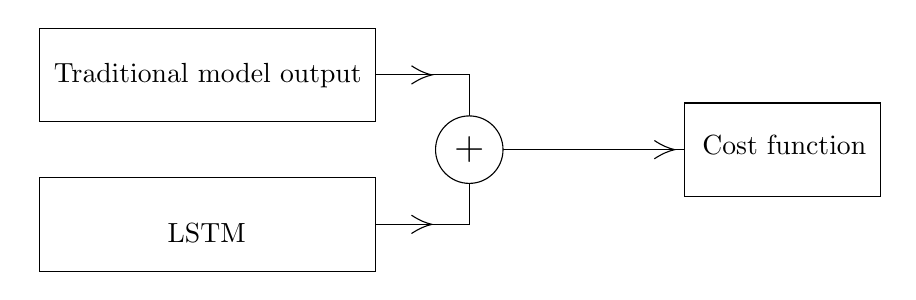
\begin{tikzpicture}[x=0.75pt,y=0.75pt,yscale=-0.9,xscale=0.9]
%uncomment if require: \path (0,300); %set diagram left start at 0, and has height of 300

%Shape: Right Angle [id:dp6736520719365272] 
\draw   (320,50) -- (370,50) -- (370,90) ;
%Shape: Right Angle [id:dp1824696211077277] 
\draw   (370,90) -- (370,130) -- (320,130) ;
%Straight Lines [id:da5169071611896188] 
\draw    (370,90) -- (485,90) ;
\draw [shift={(480,90)}, rotate = 180] [color={rgb, 255:red, 0; green, 0; blue, 0 }  ]   (10.93,-4.9) .. controls (6.95,-2.3) and (3.31,-0.67) .. (0,0) .. controls (3.31,0.67) and (6.95,2.3) .. (10.93,4.9)   ;
\draw [shift={(350,50)}, rotate = 180] [color={rgb, 255:red, 0; green, 0; blue, 0 }  ]   (10.93,-4.9) .. controls (6.95,-2.3) and (3.31,-0.67) .. (0,0) .. controls (3.31,0.67) and (6.95,2.3) .. (10.93,4.9)   ;
\draw [shift={(350,130)}, rotate = 180] [color={rgb, 255:red, 0; green, 0; blue, 0 }  ]   (10.93,-4.9) .. controls (6.95,-2.3) and (3.31,-0.67) .. (0,0) .. controls (3.31,0.67) and (6.95,2.3) .. (10.93,4.9)   ;
%\draw   (336,44.92) .. controls (340.03,47.37) and (344.07,48.84) .. (348.1,49.33) .. controls (344.07,49.82) and (340.03,51.3) .. (336,53.75) ;
%\draw   (338.5,130.08) .. controls (342.53,132.54) and (346.57,134.01) .. (350.6,134.5) .. controls (346.57,134.99) and (342.53,136.46) .. (338.5,138.92) ;

% Text Node
\draw    (140,25) -- (320,25) -- (320,75) -- (140,75) -- cycle  ;
\draw (230,50.2) node   [align=left] {\begin{minipage}[lt]{122.67200000000003pt}\setlength\topsep{0pt}
\begin{center}
Traditional model output
\end{center}

\end{minipage}};
% Text Node
\draw    (140,105) -- (320,105) -- (320,155) -- (140,155) -- cycle  ;
\draw (229.4,134.6) node   [align=left] {\begin{minipage}[lt]{122.67200000000003pt}\setlength\topsep{0pt}
\begin{center}
LSTM
\end{center}

\end{minipage}};
% Text Node
\draw  [fill={rgb, 255:red, 255; green, 255; blue, 255 }  ,fill opacity=1 ]  (370, 90) circle [x radius= 18.06, y radius= 18.06]   ;
\draw (370,90) node   [align=left] {\begin{minipage}[lt]{16.864pt}\setlength\topsep{0pt}
\begin{center}
{\Large +}
\end{center}

\end{minipage}};
% Text Node
\draw    (485,65) -- (590,65) -- (590,115) -- (485,115) -- cycle  ;
\draw (538.6,87.4) node   [align=left] {\begin{minipage}[lt]{68pt}\setlength\topsep{0pt}
\begin{center}
Cost function
\end{center}

\end{minipage}};


\end{tikzpicture}

.tex}
\caption{A sketch of how a simple hybrid model could be implemented. The traditional model and the LSTM model are completely separate, making it unnecessary to calculate gradients for the traditional model. The idea here would be for the LSTM model to learn the phenomena lacking in traditional models.}
\label{figure simple hybrid}
\end{figure}
Building from the work in this thesis there are several ways forward. We believe 
these ways forward can be categorized into two categories:
\begin{enumerate}
    \item Focus on improved machine learning results. If one is more interested in results than in understanding the underlying physics, this is the way forward. Some strategies could be:
    \begin{itemize}
        \item As mentioned several times in this thesis the only way to show that a machine learning model performs well in a specific use case is to do extensive empiric research. This means that a similar analysis needs to be performed on similar data from different sources. Going further with this would then mean to find or create a new dataset with different data sources than \citet{CAMELS_GB} or \citet{CAMELS_US}. During the initial research phase of this thesis we discovered that there was an effort in Chile to create a similar dataset \citep{CAMELS_CL}. The dataset did not seem to be of the same quality as what was used in this thesis so we decided it was out of scope to try and manage that as well.
        \item The scope of this thesis work was limited to LSTM models only. LSTM models have as mentioned in chapter \ref{LSTM drawbacks} some drawbacks that could lead one into trying a different machine learning model. Lately Convolutional Neural Networks (CNNs), which usually are used for image analysis, have shown promising results on time series data as well. \citationneeded CNNs are much more parallelizable algorithms than RNNs \citationneeded and could prove to be more efficient at doing training and prediction.
        \item In addition to CNNs, the field of natural language processing has now shifted some of the focus on LSTMs away in favour of a type of machine learning models known as Transformers \citep{transformers}. This is also to better model long-term dependencies without the computational limitations of recurrent neural networks.
        \item An often overlooked but in fact very important aspect of machine learning models is the tuning of hyperparameters. As mentioned in \ref{Method Drawbacks or something} the approach in this thesis is perhaps not thorough enough. To the author's best knowledge the best way to tune hyperpameters is in fact using a method called nested cross validation \citationneeded. This would take too long to train to be a viable approach for our work, but should be looked into in the future.
    \end{itemize}
	\item Focus on Physics. The results of this thesis are together with works such as \citet{lstm_first_paper}, \citet{lstm_second_paper} and \citet{lstm_third_paper} indicators of the possibility for using data science to better understand the relationships between easily obtainable metadata and the physics of hydrological models.
	\begin{itemize}
		\item Reducing the scope of the machine learning model to model a small effect in a classical physics-based hydrological model instead of modelling the entire system could be a way to better analyze a specific effect. Implementing the modelling of melting frozen soil, which is a physical effect currently not very well understood, could for example be a good place to start. The reason this was not tried in this thesis is that it likely requires gradients of a physical model, as this melting effect is used further down in a model. This either significantly slows down training because of a large use of automatic differentiation or requires numerical derivation, which could lead to instability.
		\item A simpler way of hybrid modelling that we wish we had the time for in this thesis could be to "model the error". This means training a model with a modified cost function where it also takes the input from a physical model. This could give a better indication of what information in the data is the most important and not properly utilized in traditional models. A simple illustration of this concept is shown in Figure \ref{figure simple hybrid}. A good place to start here would be on the CAMELS dataset, as it already contains model outputs from SAC-SMA and other (?) models \citep{CAMELS_US}. To get out of sample predictions one would have to run the traditional models themselves, though, as the dataset only contains predictions on in sample basins split time series-wise.
	\end{itemize}
\end{enumerate}
